\chapter{Bilan du projet}

\section{Autocritique}
Nous avons pu valider quatre fonctionnalités parmi celles qui étaient prévues au départ dans le cahier des charges.
\begin{itemize}
\item Créer le moteur de jeu de rythme avec Unity, et un jeu l'utilisant
\item Rendre l'application jouable sur tous les supports
\item Créer d'autres mini-jeux utilisant le moteur
\item Créer un moteur de tutoriels, et créer les tutoriels pour les jeux
\end{itemize}

\paragraph{}
Les trois premières fonctionnalités sont les plus importantes et donc nécessaires à la réussite du projet. Elles ont été implémentées avec succès.

\paragraph{}
Cependant, plusieurs idées initiales ont dû être abandonnées en cours de projet. Le principe de la "planète d'accueil" que le joueur devait personnaliser grâce aux objets qu'il aurait gagnés dans les mini-jeux, ainsi que le niveau qui se joue à l'infini, n'ont pas étés développés. En effet, après avoir réalisé l'ampleur de la tâche que représentait la création d'un seul mini-jeu, de sa conception, jusqu'à son intégration finale avec le moteur, nous avons décidé de nous impliquer pleinement dans ce processus afin d'obtenir des mini-jeux ergonomiques et cohérents pour un utilisateur. C'est ainsi que plusieurs prototypes de mini-jeux n'ont pas dépassé le stade de la conception, car jugés peu compréhensibles pour le type de gameplay facile et amusant que nous désirions.

\begin{figure}[H]\centering
   \begin{minipage}{0.49\textwidth}\centering
     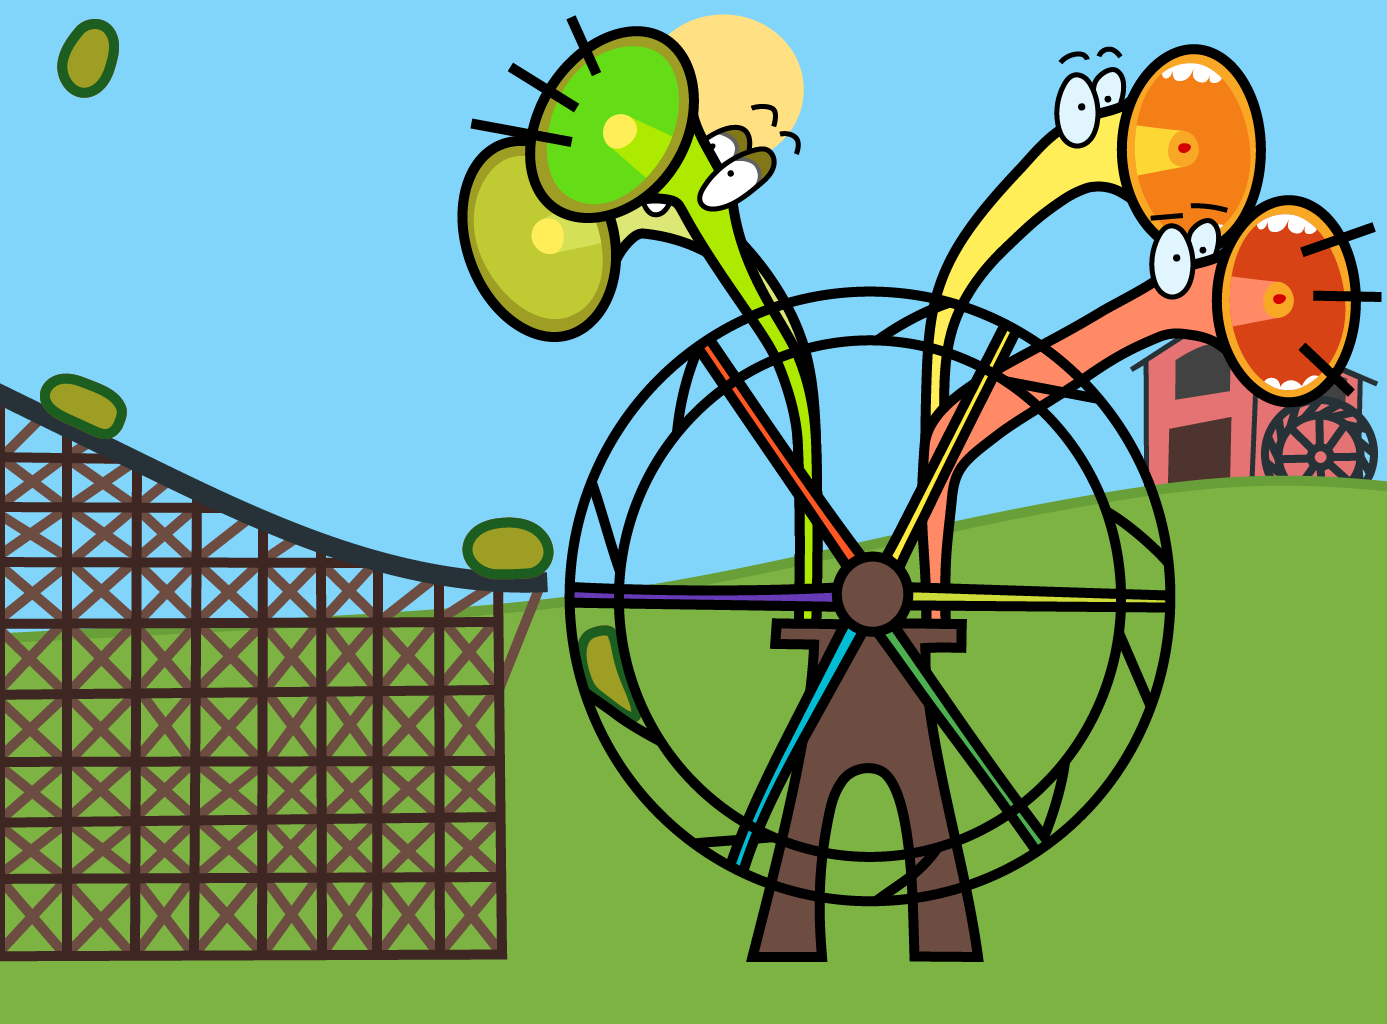
\includegraphics[scale=0.1]{./img/concept_moulin.png}
     \caption{Concept du jeu du moulin}
     \label{jeu_concept1}
   \end{minipage}
   \begin {minipage}{0.49\textwidth}\centering
     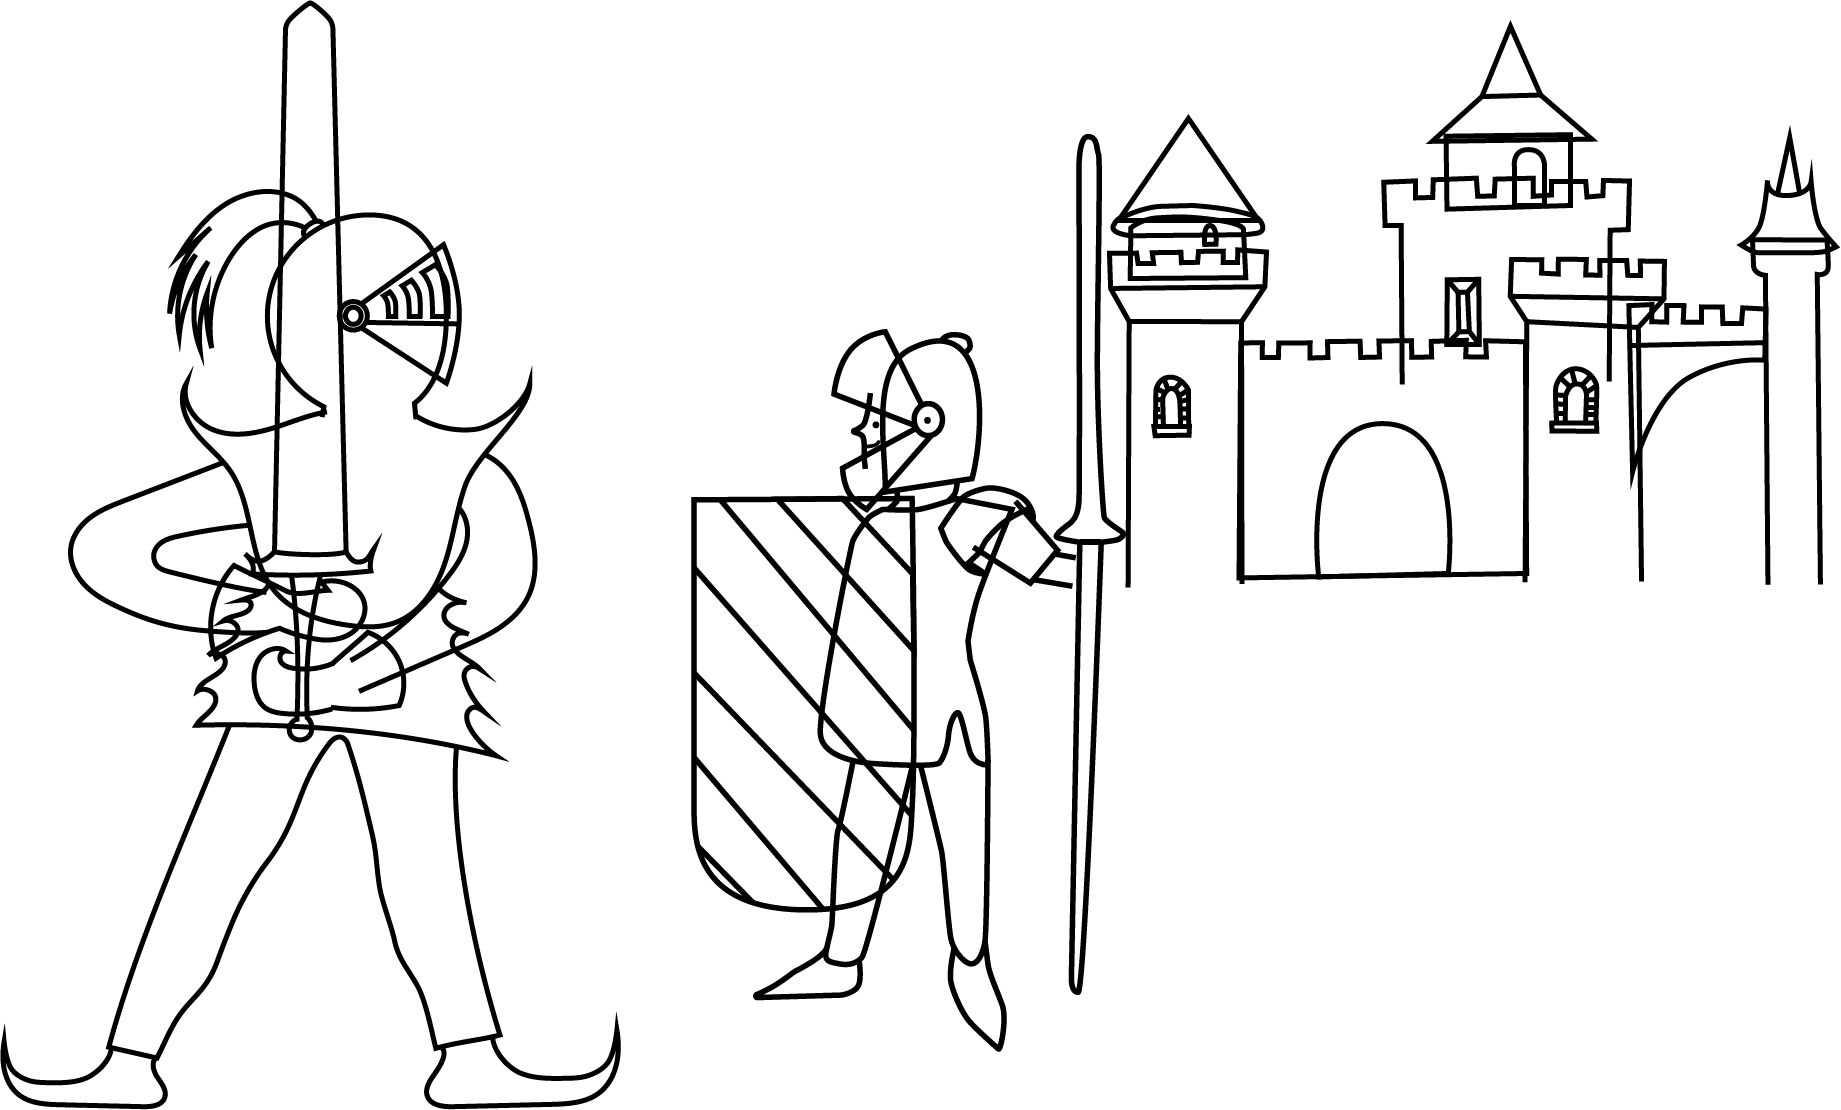
\includegraphics[scale=0.1]{./img/concept_chevalier.png}
     \caption{Concept d'un jeu de chevaliers}
     \label{jeu_concept2}
   \end{minipage}
\end{figure}

\paragraph{}
Le principal objectif que nous nous étions fixé au sein du groupe était d'avoir une application fonctionnelle, propre, bien codée et en ligne. Cet objectif est accompli, l'application est fonctionnelle et présente sur les marchés d'applications pour les systèmes Android et Apple.

\paragraph{}
Nous sommes globalement satisfaits de notre gestion du temps, et nous pensons que notre organisation y a beaucoup contribué.
L'expérience de créer un jeu de A à Z nous a beaucoup appris et nous a permis de mettre en oeuvre beaucoup de concepts sur la gestion de projets.

\section{Enseignements tirés}
Les difficultés que nous avons rencontrées tout au long du développement de l'application nous ont permis de tirer des leçons et de gagner de l'expérience.

Dans un premier temps, la maitrise de l'environnement d'Unity nous a demandé beaucoup de temps, et pour cela nous avons créé de nombreuses scènes de test au démarrage du projet afin de pouvoir nous familiariser avec l'outil, avant de commencer à travailler sur le véritable projet. Malgré ces précautions, nous avons rencontré quelques difficultés sur le développement principal. Ainsi, en travaillant en collaboration, via GitHub, nous avons constaté qu'il est impossible de travailler à deux en même temps sur la même scène, Unity ne sachant pas gérer la fusion de deux scènes. Pour résoudre ce problème, nous avons dû travailler sur des copies de scènes en leur donnant des noms de version. D'autres difficultés liées à Unity sont apparues, comme la non-compatibilité entre les versions ou la nécessité d'utiliser Windows. De plus, Unity est un logiciel demandant beaucoup de ressources, ce qui a posé des petits problèmes d'efficacité lorsque nous nous retrouvions en groupe pour travailler, avec des ordinateurs portables aux capacités de calculs faibles pour travailler efficacement.

Du point de vue du travail en équipe, nous avons dû apprendre à mieux connaitre les capacités de chacun afin d'être efficaces sur l'organisation. L'avantage d'avoir passé du temps à analyser le projet avant de commencer à le développer, est que nous avons pu choisir les activités sur lesquelles nous étions chacun le plus performant.

\paragraph{}
Ce projet a été un challenge pour nous quatre, qui nous a conduits à un véritable enrichissement.


\section{Perspectives}
Ce projet peut avoir un avenir et continuer à être développé. La base étant créée, il est possible d'y ajouter autant de mini-jeux que nécessaire, il suffit de suivre simplement la démarche que nous avons appliquée pour créer chaque niveau. Il est aussi possible de rajouter de nouvelles fonctionnalités, telles que des options communautaires, ou la possibilité d'ajouter du contenu personnalisé créé par les joueurs. Néanmoins, l'ajout de telles fonctionnalités nécessite d'avoir un contenu de base solide.

Ainsi, en fournissant un travail conséquent, l'application peut avoir la possibilité  de devenir virale, ce qui nous pousserait à développer un système monétaire en jeu, incitant les joueurs à dépenser de l'argent réel pour obtenir un avantage, ou une apparence différente.

\paragraph{}
Les perspectives de développement de cette application sont donc multiples, et l'expérience acquise durant ce projet nous permet d'affirmer qu’elles sont réalisables dans des temps honnêtes.

